\documentclass{article}
\usepackage{amsmath}
\usepackage{wasysym}
\usepackage[margin=1in]{geometry}
\usepackage{amsthm}
\usepackage{braket}
\usepackage{microtype}
\usepackage{amssymb}
\usepackage{listings}
\usepackage{tikz}
\usetikzlibrary{trees}
\newcommand{\Mod}[1]{\ (\mathrm{mod}\ #1)}
\begin{document}
\title{Artifical Intelligence Problem Set 2}
\date{}
\author{Willie Yee}
\maketitle
\noindent
\textbf{Problem 1.}\\
A. Show the complete state space for this example.\\
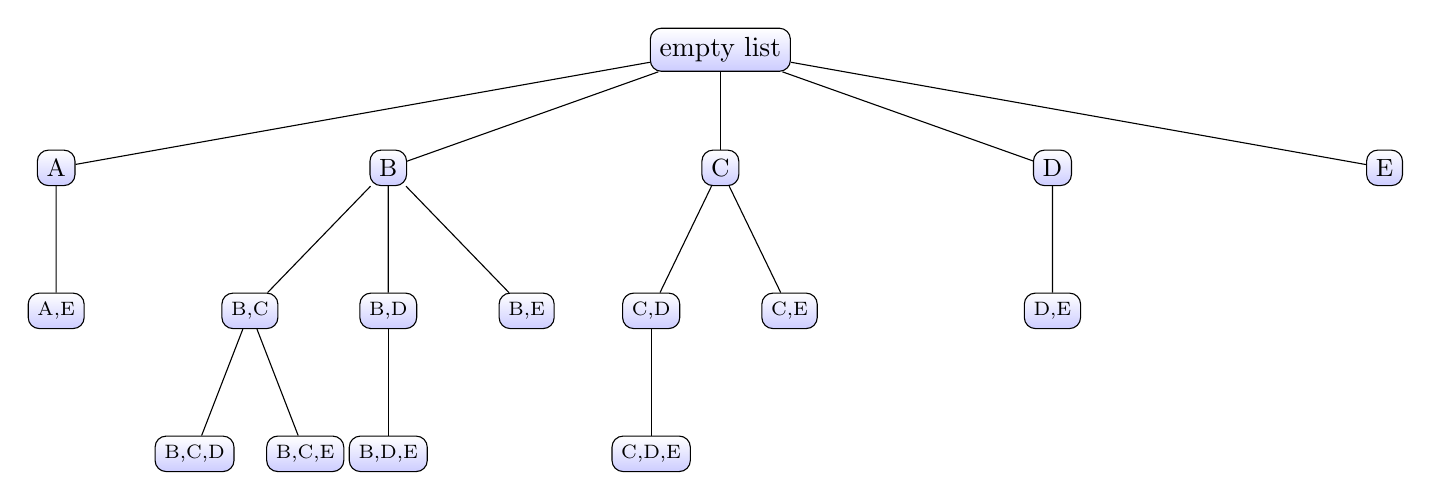
\begin{tikzpicture}[level 1/.style = {sibling distance=12em,font=\small}, level 2/.style = {sibling distance=5em,level distance=12ex,font=\scriptsize}, level 3/.style = {sibling distance=4em}, every node/.style = {shape=rectangle, rounded corners, draw, align=center, top color=white, bottom color=blue!20}]
\node {empty list}
	child { node {A}
		child { node {A,E} } }
	child { node {B}
		child { node {B,C}
			child { node {B,C,D} }
			child { node {B,C,E} } } 
		child { node {B,D}
			child { node {B,D,E} } }
		child { node {B,E} } }
	child { node {C}
		child { node {C,D}
			child { node {C,D,E} } }
		child { node {C,E} } }
	child { node {D}
		child { node {D,E} } }
	child { node {E} };
\end{tikzpicture}\\
B. Suppose that you use a depth-first search to explore the state space. Which of the states in (A) will you generate, and in what order?\\
If we depth-first search until we find a goal state, we will generate the following states, in order: (A), (A,E), (B), (B,C), (B,C,D).\\
\\
C. Suppose that you use a breadth-first search to explore the state space. Which of the states in (A) will you generate, and in what order?\\
If we breadth-first search until we find a goal state, we will generate the following states, in order: (A), (B), (C), (D), (E), (A,E), (B,C), (B,D), (B,E), (C,D), (C,E), (D,E), (B,C,D).\\\\
\textbf{Problem 2.}\\
Is the state space a tree? Yes.\\
\\
The upper bound on the depth of the state space is the total number of objects N.\\
\\
Branching factor is the number of objects still left in the pack minus the current weight that we are carrying at the moment.\\
\\
Is the depth of the shallowest goal known in advance? No, because from problem 1, we notice that neither the most valuable object nor the object with the most value to weight ratio are in the solution. This means that there could be a lot of small weight objects in the solution (high depth), or there could be a singular object that is the shallowest goal state (low depth).\\
\\
\textbf{Problem 3.}\\
A. How can you solve this problem using state space search? Give a precise description of the state space involved: What is a state, what is the successor to a state, what is a start state, how do you recognize a goal state? The state space that you describe should be a tree.\\
We can search through the state space described below to solve this problem. A state for this problem is an alphabetical list of the objects such that all elements in the list are connected to each other (assuming that any given single element objects is connected to itself). the successor to a given state is one such that the new element added to the given state is connected to all elements in the given state. The start space state is the empty list. Recognizing a goal state is simple: if the state space has K elements in the list, it is a goal state.\\
\\
B. Do you know in advance the depth of the goal states? Which search algorithm would be best: DFS, BFS, or iterative deepening?\\
The depth of the goal states is at depth K, assuming that the depth of the start space (empty list) is 0. That means the best way to search for goal states would be DFS or iterative deepening. As I do not know much about iterative deepening, I suggest DFS to be a safer and surefire way to get a goal state.\\
\\
C. Suppose that you have a graph G with V vertices and that no vertex in G has more than Q edges connected to it. That is, Q is the maximum number of edges that all connect to the same vertex. In the graph in the diagram, vertex D has 6 edges connected to it, and no other vertex has more than 6, so Q=6. Give mathematical expressions in terms of the quantities V, K, and Q for (i) the depth of your state space; (ii) the branching factor of the state space; (iii) an upper bound on the size of the state space.\\
i. Depth of the state space = K, assuming start space (empty list) is depth 0\\
ii. Branching factor is upper bounded by Q, in other words it is $\leq Q$. In general, it is equal to the maximum degree of all the elements in the list.\\
iii. The largest state space would be the case where the G is the complete graph of V vertices. We have $Q=V-1$. Thus the number of state spaces is can be summed up per level: The root of the state space has 1 element, then there are $V\choose 1$ elements in the next level of the state space and so on. Thus we have an upper bound of 
\begin{align*}
	1+{V\choose 1}+{V\choose 2}+\cdots + {V\choose K}&={V\choose 0}+{V\choose 1}+\cdots +{V\choose K}\\
	&=\sum_{i=0}^{K}{V\choose i}
\end{align*}
\end{document}